\documentclass[11pt,a4paper]{article}

\usepackage{tikz}
\usetikzlibrary{switching-architectures}


\begin{document}
Clos network with 9 modules in the first stage and 3 modules in the last stage:

\begin{center}
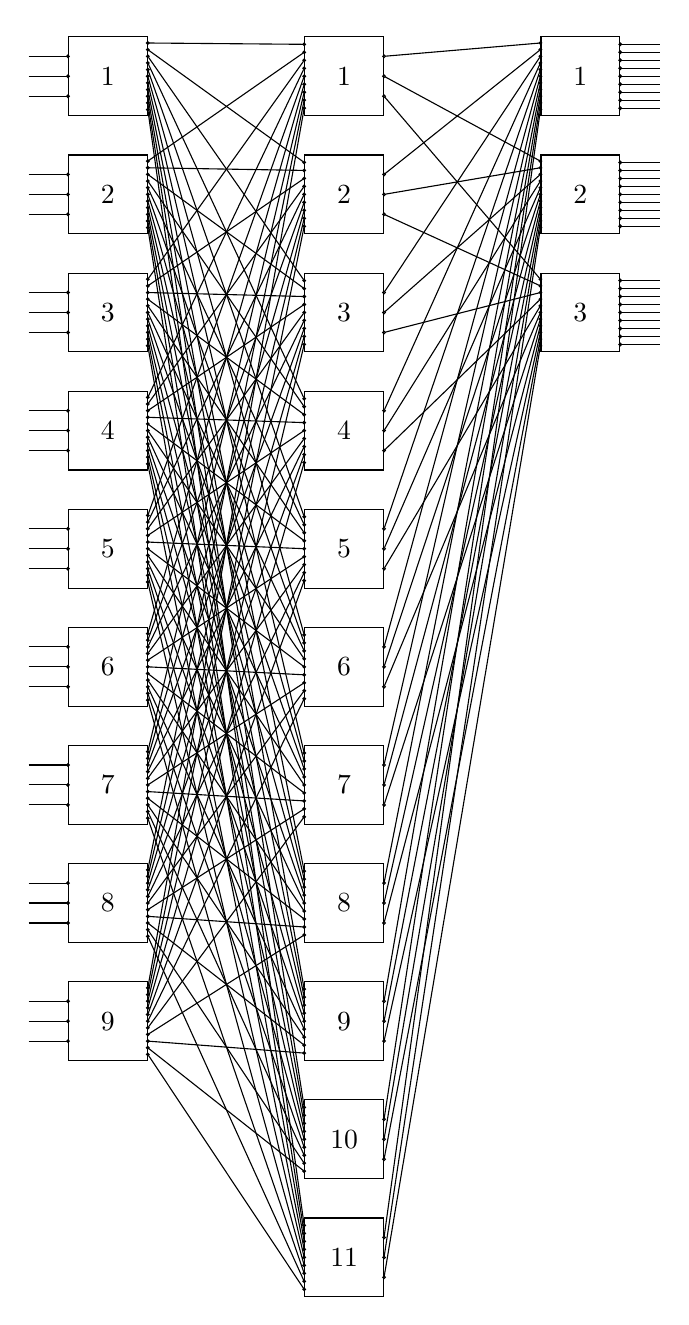
\begin{tikzpicture}
\node[N=27,M=27,r1=9,r3=3,clos snb] {};
\end{tikzpicture}
\end{center}

\newpage
Clos network with 4 modules in the first stage and 4 modules in the last stage:

\begin{center}
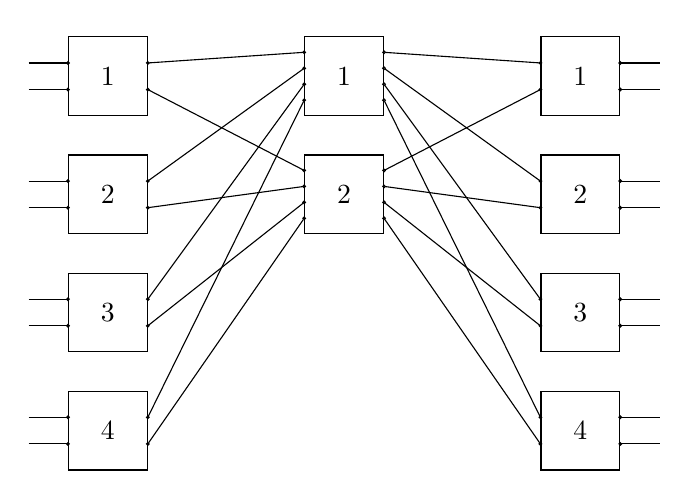
\begin{tikzpicture}
\node[N=8,M=8,r1=4,r3=4,clos rear] {};
\end{tikzpicture}
\end{center}

Example of network with labels:

\begin{center}
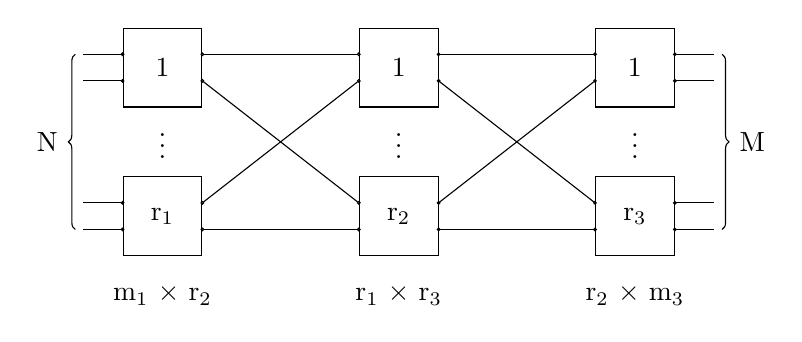
\begin{tikzpicture}
\node[clos example with labels]{};
\end{tikzpicture}
\end{center}

A simple Benes Network:

\begin{center}
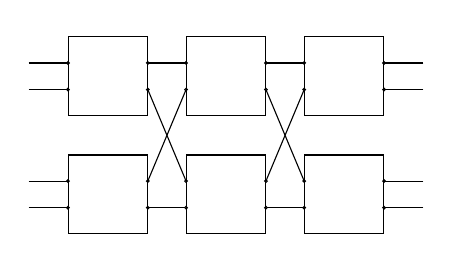
\begin{tikzpicture}
\node[P=4,benes={module label opacity=0}]{};
\end{tikzpicture}
\end{center}

A very complicated Benes Network complete $256\times 256$:
\begin{center}
\tikzset{module size=0.45cm,pin length factor=0.3,
module ysep=0.775, module xsep=4}
\scalebox{0.425}{
\begin{tikzpicture}
\node[P=128,benes complete]{};
\end{tikzpicture}
}
\end{center}


\end{document}
